\documentclass[11pt,a4paper]{memoir}
\usepackage[utf8]{inputenc}
\usepackage[english]{babel}
\usepackage{tabularx}
\usepackage{amsmath}
\usepackage{amsfonts}
\usepackage{amssymb}
\usepackage{graphicx}
\usepackage{chemmacros}
\usepackage{chemfig}
\usepackage{gensymb}
\author{Benjamin Chalmers}
\title{A Level Chemistry OCR A 2015}
\addto\captionsenglish{%
 \renewcommand\chaptername{Module}}
\newcommand*\conj[1]{#1}
\newcommand*\mean[1]{\bar{#1}}

\begin{document}


\frontmatter
\maketitle
\newpage
	This is a series of rough notes for the new spec examinations in Chemistry. They will not be whole and I will be skimming over areas of the course that I know well.
	
	I will be writing this using the specification as my guide. H032 is the course and you can find the original document through Google. This document will be continuously referencing this spec so if you are wondering what all the references are too.
\newpage
\tableofcontents
\mainmatter

\chapter{Practical Skills in Chemistry}
	Practical skills are crucial to chemistry.
	Chemistry is a practical subject; as such we should understand how to correctly carry out our experiments.
	Practical skills are a recurring theme throughout the other 4 modules so a good knowledge of these skills is vital to success.

\section{The doing 1.1.1 \& 1.1.2}
	\paragraph{Planning} is a crucial to any and all experiment doing.
	In this course you should be able to do several things with ease.
	
	Firstly you should understand the range of equipment available and there appropriate usage.
	You should then have the mental capacity to apply this knowledge to a given situation and, in so doing, design a practical.
	This understanding comes with time and I will not go into much detail.
	
	Secondly you should understand these distinctions.
	\textit{Independent} variables are ones which the experimenter changes e.g. the temperature of the heater.
	\textit{Dependent} variables depend on the independent ones and are measured e.g. the amount of gas released from the reaction.
	\textit{Control} variables are ones which remain constant and are controlled by the experimenter e.g. the amount of substance added.
	
	Because I like maths think of it like this. Let y be the dependent, x be the independent and c be the control/constant:
	
	\begin{center}
	\[y= f(x) + c\]
	\end{center}
	
	By keeping c constant and changing x we can derive $f(x)$ which is what many experiments try to do.
	Determining the relationship between the independent and the dependent variable.
	
	Lastly you should be able to evaluate the experimental method to determine whether or not it is appropriate to find the expected outcomes.
	This part requires critical thinking and an understanding of modules 3-4
	
	\paragraph{Implementing} is more about usage.
	I will not go into it fully here but here is an overview.
	
	You need to know your units, techniques and how to use the apparatus.
	Ask your teacher to show you the techniques and how to use the apparatus.
	The units will be visited as we explore the rest of this spec.
	
\section{The reviewing 1.1.3 \& 1.1.4}
	
	\paragraph{Reviewing} is necessary, it comprises two parts, that of analysis and of evaluation.
	
	\paragraph{Analysis} simply the processing and interpretation of qualitative\footnote{Observed data e.g. colour and effervescence} data combined with an understanding of the maths skills involved to explore quantitative\footnote{Data that is measured with a numeric output e.g. temperature} data.
	Basic statistics skills required are as follows:
	
	\begin{center}
		\begin{equation}
		\mean{x} = \frac{\sum_{i=1}^n x_i}{n}
		\end{equation}
		\textit{Technically not necessary but makes your PAGs feel more exact:}
		\begin{equation}
		y=a + bx \newline
		b=\frac{n\sum_{i=1}^n x_iy_i - \sum_{i=1}^n x_i \sum_{i=1}^n y_i}{\sum_{i=1}^n x^2_i -(\sum_{i=1}^n x_i)^2} \newline
		a = \mean{y} - b\mean{x}
		\end{equation}
	\end{center}
	
	Plotting graphs is important because this exam uses mostly graphical methods to find things such as gradients (which, at a point, it the gradient of the tangent to the curve often expressed as $\frac{dy}{dx}$).
	Just remember to use a good scale when drawing them.
	
	\paragraph{Evaluation} is the process in which we look back at the plan and the method and, well, evaluate it.
	You need to understand the limits of the procedure used, identifying anomalies and refine the experimental design by suggesting improvements to the procedures and apprentice.
	
\chapter{Fundementals in chemical semantics}
    This chapter acts as a bridge between A level and GCSEs. It is quite       simple with a lot of practice of molar equations, percentages and           remembering through rote learning.
    

\section{Fundamentals in chemical semantics 2.1.1}
	\paragraph{Isotopes} are the same elements (same number of protons/atomic number), but with a differing numbers of neutrons. This gives it a different mass number.
      
	Chemists compare the masses of subatomic particles using relative masses.
	This is where where we look at the mass of these particles relitive to $\frac{1}{12}$ the mass of $^12$C
	
\begin{tabular}{ |p{3cm}||p{3cm}|p{3cm}|p{3cm}|  }
 \hline
 Particle    & Abbreviation &Relative charge&Relative mass\\
 \hline
 Proton   & p+    &1+&   1\\
 Neutron& n  & 0   &1\\
 Electron& e-  & -1& 0.0005\\
 \hline
\end{tabular}

\paragraph{Charge} comes from atoms, or molicules, wich are defficient in, or have a surplus of electrons.
Given that protons have a charge of +1 and electrons have a charge of -1 to have zero overall charge we need the same number of electrons as there are nutrons, this is the most stable state.

\paragraph{Atomic Numbers}show the number of protons in an element. These are then used to order the elements in the periodic table. For example, $_{2}$Li or $_{8}$O.

\paragraph{The Mass number} is the number of protons + number of neutrons. The \textbf{atomic number} is the \textbf{number of protons} only.
An ion is a charged atom i.e. lost or gained electrons.

\paragraph{The Relative isotopic mass}is the mass of an isotope compared to \(\frac{1}{12}th\)\\ of a carbon-12 atom. In questions assume this is equal to the mass number.

\paragraph{The relative atomic mass}is the \textbf{weighted mean} mass of an atom relative to  \(\frac{1}{12}th\)\ the mass of a carbon-12 atom. The weighting takes into account \textbf{percentage abundance and relative isotopic mass}. 

\paragraph{To determine} percentage abundance and relative isotopic mass of an element, they are found experimentally using a mass spectrometer. You do not need to know how it works, but if you want, it's mentioned in the OCR A chemistry textbook.
\[m/z= \frac{Relative Mass Of Ion}{Relative Charge}\]\
\paragraph{The relative isotopic mass} is found on the x-axis and percentage abundance by the peak e.g. if there is 75.78\% of CL-35 and 24.22\% of Cl-37, you would do this:
\[Relative Atomic Mass=\frac{(75.78*35)+(24.22*37)}{100}\]\
Where 75.78x35 is the contribution from Cl-35, 24.22x37 is the contribution from Cl-37 and 100 is the max percentage. Questions like to ask you to guess what the elementn is by its mass, so make sure you are confident in this skill. 
\paragraph{For simple molecules}, the term relative molecular mass will be used.
For compounds with \textbf{giant} structures, the term relative formula mass will be used.
\section{Compounds, formulae and equations 2.1.2}
\begin{tabular}{ |p{3cm}||p{4cm}||p{3cm}||p{3cm}|  }
 \hline
 +1    & 1- &2-&3-\\
 \hline
 Ammonium \[ NH_4^+ \]    & Hydroxide \[OH^-\]    &Carbonate \[CO_3^ 2-\]& Phosphate \[PO_4^ 3-\]\\
 N/A& Nitrate \[NO_3^-\]  & \[SO_4^{2-}\]  & N/A\\
 N/A& Nitrite \[NO_2^-\]  & Sulphite \[SO_3^{2-}\]& N/A\\
 \hline
 N/A & Hydrogencarbonate \[HCO_3^-\] & Dichromate(VI) \[Cr_2O_7^{2-}\] & N/A\\
 \hline
 N/A & Manganate(VII)/ Permanganate \[MnO_4^-\] &N/A&N/A\\
 \hline
\end{tabular}
\section{Amount of substances 2.1.3}
\subsection{1.The mole}
\paragraph{The amount of substance},n, is used to count the number of particles in a substance- measured in moles. One mole contains \textbf{\(6.02*10^{23}\)} particles- known as \textbf{Avogadro's constant}.
\paragraph{Molar mass} /\(M_r\) is the mass per mole which is why its units are \(gmol^{-1}\) e.g. carbon has a molar mass of 12, where 1 mole is 12 grams.
\newline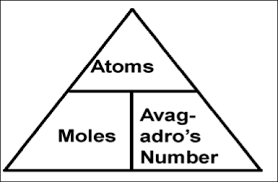
\includegraphics[scale=1.0]{atms_triangle}
\paragraph{A mole of gas} fills, in standard conditions (RTP), 24.0 dm3 of space. The number of moles is directly proportional to the space filled. You can find this information on the formula sheet under “Molar gas volume”.
\paragraph{When the substance isn’t under standard conditions} the ideal gas equation is used, \(pV=nRT\). They give us a number called the Gas constant- 8.314 J/mol/K. This value is given on the formula sheet, however you have to know non-SI units and working it out takes longer than remembering this figure.
\subsection{2.The determination of formulae}
\paragraph{Empirical Formula} is the simplest whole number ratio of atoms of each element present in a compound.
\paragraph{Molecular formula} is the number and type of atoms of each element in a molecule e.g. \(H_2SO_4\) .
\paragraph{The determination of formula} is a necessary part of this exam. They love questions along the lines of:
\begin{enumerate}
\item “Raheem has found that his substance has a composition by mass of  23.3% magnesium, 30.7% sulfur and 46.0% oxygen "
\begin{itemize}
\item (a) Work out the empirical formula
\end{itemize}
\end{enumerate}
\paragraph{It is assumed} that the percentage composition of the element is equal to the mass of the element e.g. 23.3\% is 23.3g. We also know the \(M_r\) of each element:
\begin{itemize}
\item Magnesium is 24.3 \(gmol^{-1}\)
\item Oxygen is 16 \(gmol^{-1}\)
\item Sulfur is 32.1 \(gmol^{-1}\)
\end{itemize}
\paragraph{Next, you find the moles} by dividing the mass by the \(M_r\). 
\newline Therefore:\(\frac{23.3}{24.3}\) = 0.959, \(\frac{30.7}{32.1}\) = 0.956 and \(\frac{46.0}{16}\) =2.875. Then you divide by the smallest number of moles, giving the empirical formula. 0.959/0.956=1, 0.956/0.956=1 and 2.875/0.956=3. This makes the empirical  formula: \(MgSO_3\) .
\paragraph{In other cases}, they may ask you tork out the molecular formula using the empirical formula and the molecular mass given in the question. For example:
"Fatima found that a substance had a percentage composition of 40.0% carbon, 5.7% hydrogen and 53.3% oxygen has an atomic mass of 175 g/mol. What is the molecular formula?"
\paragraph{To minimise my working,}I shall provide you with the empirical formula \ch{CH_2O}. You can try to work out how I did this using the method above.
\paragraph{In order to work out the molecular formula} you need a little algebra. As we know the Mr is 180 and the empirical formula is \(CH_2O\) - Mr 30,as we want to work out the number of each atom you would do:
\newline \[180=30x\] \[\Delta\\x=6\]
\paragraph{Finally,} you multiply the atoms present in the empirical formula by 6 from the above equation. This gives a molecular formula of \(C_6H_{12}O_6\) .
\paragraph{Hydrated salts} are calculated in much the same way. They are expressed
like this CuSO4·nH2O and you will be given some numbers to workout n.These are likely the mass of water and mass of anhydrous salt .
\newline Heating a substance removes the H2O making it anhydrous. To Hydrate simply dissolve the salt in water and evaporate the water very slowly.(see pg.24 in book).
\subsection{How accurate is experimental formula?}
\paragraph{You need to make an assumption that all water is lost}. You can only see the surface of the crystals; the inside is unknown to us, so water could be found there. To \textbf{reduce error, you should heat to a constant mass}- when mass no longer changes when heated. rthis means you can be sure that it is anhydrous.
\paragraph{You also assume there is no further decomposition}. Many salts decompose further when heated e.g. \(CuSO_4\) turns into black copper(III) oxide.
\subsection{3.Calculation of reacting masses, gas volumes and mole concentrations}
\paragraph{You need to know}all the calculations using liquids, gases and solids to find moles. You also need to know how to convert between \(gdm^{-3}\) and \(moldm^{-3}\) . You just need to remember that when you convert from \(moldm^{-3}\) you just multiply by Mr.
\newline
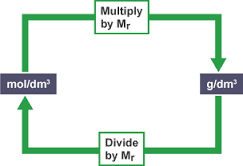
\includegraphics[width=0.85\textwidth]{chem1.png}
\newline You will also need to know how and when to use the ideal gas equation:
\begin{equation}
pV=nRT
\end{equation}
\begin{center} p= Pressure in Pa

 V= Volume in \(m^3\) 

n= moles

R= ideal gas constant(8.314 \(Jmol^{-1}K^{-1}\) ) 

T= temperature(K) 
\end{center}
\paragraph{With the ideal gas equation} you assume that: no intermolecular forces;sizes are negligible; random motion and elastic collisions.
You will also need to remember how to convert between the units as questions sometimes try to trick you. These are listed here:
\begin{itemize}
\item \(cm^3\) to \(m^3\) = \(*10^{-6}\)
\item \(dm^3\) to \(m^3\) = \(*10^{-3}\)
\item \degree C to K = +273
\item kPa to Pa = \(*10^3\) 
\item 1 atm = 101kPa = 101000 Pa
\end{itemize}
\newpage
\begin{equation}
Percentage Yield= \frac{Actual Yield}{Theoretical Yield}\\
\end{equation}
\newline
\begin{equation}
Atom Economy= \frac{\sum Mr(desired) prod}{\sum Mr All Prod}\\
\end{equation}
\paragraph{Percentage yield} doesn't really allow 100\% in real life because: the reaction \textbf{may not have fully taken place};\textbf{side reactions occur} and \textbf{purification} leads to loss in product.
\%age yield is in reference to the percentage of the theoretical yield that was actually yielded i.e. actual yield. Atom economy simply refers to the number of wasted atoms (atoms that form waist products).
\section{Acids 2.1.4}

	\paragraph{The acids to remember} are the following:
	\begin{itemize}
		\item HCl is Hydrogen Chloride
		\item \ch{H2SO4} is Hydrogen Sulphate
		\item \ch{NOH3} is Nitric Acid
		\item \ch{KOH} is Potassium Hydroxide
		\item \ch{CH3COOH} is Ethanoic Acid (although it is commonly called Acetic Acid).
	\end{itemize}
    Acids release \ch{H+} ions when in aqueous solution.
	To examine the strength of an acid we must look at the dissociation of the \ch{H+} ions.
	Take for example HCl. The dissociation of HCl in aqueous solution looks like this, 
	\begin{center}
		\ch{HCl(aq) -> H^+(aq) + Cl^-(aq)} 
	\end{center}
	As you can see all of the hydrogen atoms have dissociated.
	This would make HCl a \textit{strong acid}. 
	
	Where the \ch{H+} ions only partially dissociate we call it a \textit{weak acid}. Take Ethanoic acid, its dissociation in aqueous solution looks like this, 
	\begin{center}
		\ch{CH3COOH(aq) <=> H^+(aq) CH3OO^-(aq)}
	\end{center}
	 As we can see the \ch{H+} ions haven't entirely dissociated.
	 The \ch{<=>} implies that the reaction is incomplete and forms an equilibrium, so the acid hasn't completely dissociated.
	
	There is a point to be made that not all ionic compounds with hydrogen atoms are acids.
	It is only those compounds that form \ch{H+} ions when dissolved in aqueous solution that we call acids.
	
	\paragraph{The common bases} are metal oxides, metal hydroxides, metal carbonates and ammonia, \ch{NH4}.
	Bases neutralise an acid to form a salt.
	
	\paragraph{An Alkali} is a special type of base which, when dissolved in water, releases hydroxide ions.  They are also known as soluble bases.
	For example take the base \ch{Mg(OH)2},
	\begin{center}
		\ch{Mg(OH)2(s) + aq -> Mg^{2+}(aq) + 2 OH-(aq)}
	\end{center}
	We can see that \ch{Mg(OH)2} is an alkali as it releases \ch{OH-} ions when dissolved in aqueous solution.
	
	\paragraph{The alkali and base to remember} are the following:
	\begin{itemize}
		\item \ch{NaOH} is Sodium Hydroxide
		\item \ch{KOH} is Potassium Hydroxide
		\item \ch{NH3} is Ammonia
	\end{itemize}
    \paragraph{You need to remember} that:
   \begin{itemize}
\item\ch{H+ + OH- -> H2O}, 
\item   \ch{CO3^{2-} + 2 H+ -> H2O + CO2} 
\item   and finally \ch{O^{2-} + 2 H+ -> H2O}.
	\end{itemize} 
    Using these ionic equations you should be able to form full equations.
	
	\paragraph{Titrations} are a technique to achieve a neutralisation reaction.
	We take an acid and a alkali and we slowly add one to the other using a burette.
	
	
	The preparation of a standard solution simply involves dissolving a exact and known mass of ionic compound and dissolving it in a know volume of water.
	This is done in a volumetric flask.
    \section{Redox 2.1.5}

	\paragraph{OIL RIG} is a fantastic acronym.
	Oxidation Is Loss, Reduction is gain.
	Remembering this is vital.
	If we describe a reaction as having \textit{oxidised} X, we mean to say that X has lost electrons.
	If a reaction is described as having \textit{reduced} X, we mean to say that X has gained electrons. It is important to remember \textbf{elements have an oxidation number 0.}
	
	To write a redox reaction we have equations like this:
	\begin{center}
	\vspace{7mm}
	\ch{
		2 "\OX{o1, \ox[pos=top]{0,Na}}" + "\OX{r1, \ox[pos=top]{0,Cl}}" {}2
		->
		2 "\OX{o2,\ox[pos=top]{+1,Na}}" {}+ + 2 "\OX{r2, \ox[pos=top]{-1,Cl}}" {}-
	}
	\redox(o1,o2){\small OX: $- 2\el$}
	\redox(r1,r2)[][-1]{\small RED: $+ 2\el$}
	\vspace{7mm}
	\end{center}
	We use Roman numerals to indicate oxidation numbers, memorise the following oxidation numbers:
	\begin{itemize}
		\item Oxygen has the oxidation number -2 unless in peroxide, in which case it is -1
		\item Hydrogen has the oxidation number +1 unless in a metal hydride in which case it is -1
		\item Fluorine has the oxidation number -1
	\end{itemize}
	So to work out whether a chemical has been oxidised or reduced we do the following.
	
	\begin{enumerate}
		\item Find the balanced symbol equation,
		
		\ch{2 Al + 3 H2SO4 -> Al2(SO4)3 + 6 H2}
		
		\item Then we fill in the oxidation numbers for the ones we know,
		
		 \ch{2 "\ox{0, Al}" {} + 3 "\ox{+2, H}" {}2 "\ox{-2, SO}" {}4 -> Al2 "\ox{-6,(SO}" {}4)3 + 6 "\ox{0, H}" {}2}
		 
		\item The \ch{Al2 "\ox{-6,(SO)3}" {}4} has no overall charge so the oxidation numbers must add to 0,
		
		\ch{"\ox{+6, Al}" {}2 "\ox{-6,(SO4)}" {}3}
		
		\item Now we have \ox{+6, Al}$_2$ we can see that \ox{+3, Al}. So Aluminium went from Al to \ox{+3, Al} meaning it has been oxidised in this reaction.
		
		\item The hydrogen went from \ox{+2, H}$_2$ to \ch{H2}. This is a reduction so we say hydrogen has been reduced.
	\end{enumerate}
	\paragraph{It is important}to note that when writing oxidation numbers down in exam questions, it only means for one atom of a molecule.
    In summary oxidation numbers refer to the number of electrons individual atoms in compounds have lost/gained.
	They are like charge but apply to atoms and not the overall compound.
	They are used to explain whether a reaction has oxidised an atom or reduced it.
   \newpage
   \section{Electron structure 2.2.1}

	\paragraph{Shells} are areas where there is a high probability of finding an electron.
	They are split by looking at major energy levels.
	The period an atom is in indicates how many shells it has.
	The number of electrons that can fit into a shell can be worked out by $2n^2$ where $n$ is the shell number.
	
	\paragraph{Shells are sub-divided} into sub-shells. The ones you need to know are as follows,
	\begin{itemize}
		\item s orbital which can hold 2 electrons, one in all shells
		\item p orbital which can hold 6 electrons, one in all but shell 1
		\item d orbital which can hold 10 electrons, one in all but shells 1 \& 2
	\end{itemize}
	They fill in order.
	
	\paragraph{Orbitals} are regions around the nucleus which can hold up to two electrons with opposite spin.
	This diagram is of a P orbital and the arrows indicate the spin:
    \begin{center}
    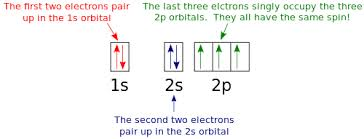
\includegraphics[scale=1]{orbital}
    \end{center}
    \paragraph{Order of fill} is as follows, 1s$^2$2s$^2$2p$^6$3s$^2$3p$^6$4s$^2$3d$^{10}$4p$^6$ in the standard format $x$s$^n$
    The examination may well ask you to write the electron configuration of an atom.
	Unless otherwise instructed, a short cut is to use a noble gas as a base.
	For example if I said write the electron configuration of sodium you can say [Ne]3s$^1$.
	You need to know how to do this for all elements up to and including Kr.
   \paragraph{Energy levels} are the reason different shells fill differently. 
   As you probably know, lower energy levels need to fill before higher ones.
   This is why,for example, the s- subshell fills before the p- subshell.
   As we go up, the shells we also ascend in energy level.
	The most interesting part is the 4s sub-shell and the 3d sub-shell.
	The 4s sub-shell and the 3d sub-shell have very similar energy levels.
	The 4s sub-shell is, however, slightly lower so the 4s fills first.
	When the 3d sub-shell fills the energy level falls meaning, the 4s fills before 3d and the 4s empties before 3d.
	This is important when looking at the electron configuration of D Block ions.
    \section{Bonding 2.2.2}
    \paragraph{Ionic bonding} is the \textbf{strong electrostatic attraction} between anions and cations.
    It usually occurs when there is a \textbf{metal cation} and a \textbf{non-metal anion}.
    \paragraph{The giant ionic lattice} is the structure of ionic compounds. 
    Each ion is surrounded by oppositely charged ions in a regular structure e.g, in NaCl , each Na$^+$ ion is surrounded by 6 Cl$^-$ ions and vice-versa.
    \paragraph{Ionic compounds have high melting and boiling points} because there needs to be high temperature in order to overcome the strong electrostatic forces between ions.
    The melting point is higher if the ionic charges are greater and the size of an ion is also a factor.
    \paragraph{Ionic compounds usually dissolve in polar solvents}such as water. Polar molecules attract and surround each ion in solution and break down the lattice e.g. NaCl dissolves in water.
    However, in ionic structure with large ionic charges, some polar solvents such as water may not be able to overcome the strong electrostatic attraction.
    \paragraph{ In a solid state, ionic structures don't conduct electricity} because the \textbf{ions} are \textbf{localised} meaning there are \textbf{no mobile charge carriers}.
    In an \textbf{aqueous state}, however, the \textbf{ions are free to move} as mobile \textbf{charge carriers} allowing electricity to be conducted.
   \paragraph{Dot-and-cross diagrams} are the same as they have always been.
	Used for drawing the simplest of ionic bonds, that of metal - non-metal.
	Just remember: the square brackets;only the outer shell is drawn and that the charge is shown as superscript.
  \pagebreak
  \paragraph{In summary} ionic compounds have these properties:
    \begin{itemize}
		\item Have \textbf{high melting and boiling points}
		\item Tend to \textbf{dissolve} in \textbf{polar} solvents
		\item Only conduct \textbf{electricity} when in \textbf{liquid} state or dissolved in aqueous solution.
	\end{itemize}
 
    \paragraph{Covalent bonding} is the strong electrostatic attraction between a shared pair of electrons and the nuclei of the bonded atoms. It occurs in:
    \begin{itemize}
	 	\item Non-metallic elements such as \ch{H2} and \ch{O2} form covalent bonds.
	 	\item Non-metallic compounds such as \ch{H2O} and \ch{CO2} form covalent bonds.
	 	\item Even polyatomic ions are covalently bonded such as \ch{NH4^+}
	\end{itemize}
    \paragraph{It can also be thought of as an overlap of orbitals} each containing \textbf{one} electron to give a shared pair of electrons. 
    This is why when drawing a dot and cross diagram for this, you draw overlapping circles with electrons shared.
    These electrons are attracted to the nuclei of both the bonded atoms.
    The bonded atoms often have the same elec. config. as the nearest noble gas.
    There are the following three types of covalent bonding that you are expected to know about,
	\begin{enumerate}
		\item Single covalent bonding, this is where there is one shared pair of electrons per nuclei.
		\item Multiple covalent bonding, this is where there are multiple pairs of shared electrons per nuclei e.g. double bond in \ch{CO2} 
		\item Dative covalent bonding, this is where the shared pair is supplied by only one of the atoms.
	\end{enumerate}
   \begin{center}
   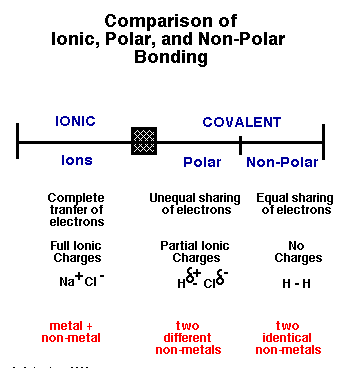
\includegraphics[scale=1]{2016-08-10}
\end{center}
   \ch{NH4^+} is a good example of a dative covalent bond. A \ch{H+} ion meets ammonia and ammonia provides the electron pair for the covalent bond.The dative covalent bond is shown by a $\rightarrow$ to the hydrogen i.e.
   \newline
    \begin{center}
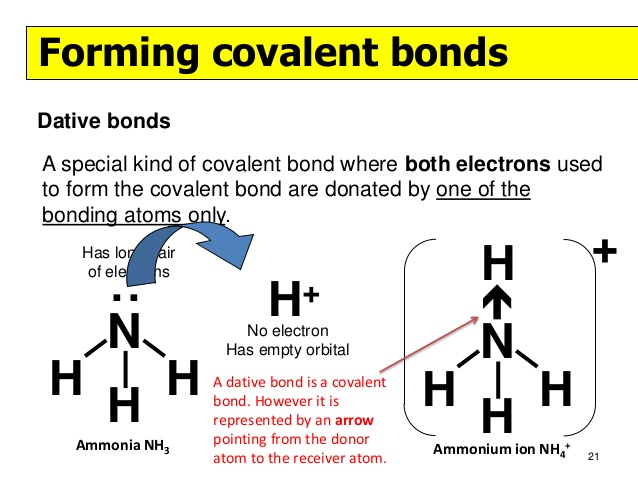
\includegraphics[scale=0.5]{ammonia}
\end{center}
\paragraph{You will need to learn}all of the types of covalent bonds. Using your GCSE or A-level textbook for any practice you require is very useful to master this skill.
	\paragraph{Average Bond Enthalpy} is simply a measure of the  covalent bond strength, take a \ch{Br-Br} \textbf{covalent} bond for example. \footnote{Note that you only need to understand the concept of avg. bond enthalpies; definitions for this are not required.}
   The larger the value of the average bond enthalpy, the stronger the covalent bond.
    \section{The shapes of simple molecules and ions 2.2.2}
	
	\paragraph{You need to know} the shapes of, and bonding angles in, molecules and ions with up to six electron pairs (including lone pairs) surrounding the central atom as predicted by electron pair repulsion.
	
	\paragraph{Electron pair repulsion} is used for explaining and predicting shapes of covalently bonded molecules as well as the relative repulsive strengths of paired and unpaired electrons.
	It works on the principle that electron pairs repel to arrange themselves around an atom as far apart as possible.
	They do this in 3D, which may sound obvious, but so far in chemistry we have worked only with 2D models.
	To draw 3D diagrams we need to understand the following standards,
	\begin{itemize}
		\item \chemfig{A-B} is used for a bond in the same plane as the paper
		\item \chemfig{A<B} is used for a bond coming out of the paper
		\item \chemfig{A<:B} is for bonds going into the plane of the paper
	\end{itemize}
    \paragraph{Lone pair} repulsion is greater than that of bond pair.
	This is because the lone pair of electrons occupy more space than the bonded pair, overall resulting in a slightly higher repulsion from the lone pair.
	The bonding angle is, therefore, reduced by around 2.5\degree for every lone pair.
	
	\paragraph{Common, and basic examples} are molecules such as, \ch{CH4} which has a bonding angle of 109.5\degree and no lone pairs and forms a tetrahedral structure; \ch{NH3} which has a bonding angle of 107\degree with one lone pair and this is pyramidal; finally \ch{H2O} which is non-linear and with its two lone pairs has a bonding angle of 104.5\degree .
	
	\paragraph{The last shapes to be familiar with} are \textit{trigonal planar} which have a bonding angle of 120\degree , \textit{linear} which are 180\degree and \textit{octahedral} which are 90\degree . 
  \section{Electronegativity and bond polarity 2.2.2}
\paragraph{Electronegativity} is the ability of an atom to attract bonding electrons in a covalent bond.	
	\paragraph{The Pauling scale} is a scale used to measure the \textit{electronegativity} of an atom. As we go right, across the periodic table, the electronegativity increases alongside a decrease in atomic radius. As we move up the table we see an decrease in the number of shells, hence a decrease in atomic radius, so we see then another increase in electronegativity. So the nearer F in the table, the higher the electronegativity.
	\paragraph{Covalent, Polar covalent and ionic} bonds are defined as the difference in electronegativity of the bonding atoms.
	Where the difference is zero we call the bond covalent/ non-polar covalent.
	Where the electronegativity difference is less than 1.8 (but greater than 0) we call it polar covalent and where it is greater than 1.8 we call it ionic.
\paragraph{Polar bonds} are covalent bonds between two elements with \textbf{unequal} electronegativities.
	\chemfig{H^{\delta +}-Cl^{\delta -}} is an example of a polar bond, and by extension a polar molecule.
	Hydrogen has a lower electronegativity than chlorine causing the chlorine in the covalent bond to become slightly negative.
	This type of bonding is called a permanent dipole.
\paragraph{Larger molecules} are interesting because we need to look at structure to see if the overall molecule is polar or non-polar(due to dipoles cancelling each other out due to their direction).
	Take \ch{H2O}, this has a non-linear structure. Both the \chemfig{H^{\delta +}-O^{\delta -}} bonds are polar and given its non-linear structure, these polar bonds don't cancel out.
	This makes \ch{H2O} a polar molecule because it has an overall \textbf{dipole- the separation of opposite charges}. It has a permanent dipole as the dipole doesn't change.
	\paragraph{However, take \ch{CO2}, a similar covalent molecule} with two \chemfig{C^{\delta +}=O^{\delta -}} polar bonds.
	But this is where it changes. The structure is linear.
	This means that the two polar bonds cancel out \chemfig{O^{\delta -}=C^{\delta +}=O^{\delta -},
	meaning that the overall molecule, in the case of \ch{CO2}, is non-polar.
    \paragraph{A bond will be non-polar when}: 
    \begin{enumerate}
\item The bonded atoms are the same- a pure covalent bond e.g. \ch{O2}
\item The bonded atoms have the same or very similar electronegativities. 
\end{enumerate}
Carbon and hydrogen have similar electronegativities- that's why hydrocarbon liquids are usually non-polar solvents and don't mix with water.

\section{Intermolecular Forces 2.2.2}
An important distinction from ionic or covalent bonding is that these are forces between different molecules rather than what holds\textit{ a molecule} together. Permanent dipole–dipole and induced dipole–dipole interactions can both be referred to as van der Waals’ forces. This is important to know if your teacher isn't aware of this change to the syllabus.

	\paragraph{Permanent dipole - dipole interactions} are caused by\textbf{ polar molecules attracting each other} and forming a permanent electrostatic interactions.
	This is quite similar to giant ionic lattices but occurs with polar covalent molecules such as water rather than ions.
	The distinction is that it is \textbf{between separate molecules} e.g. water molecules. See the example below:
    \begin{center}
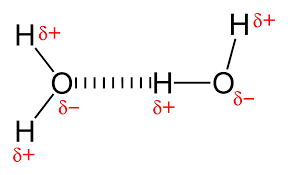
\includegraphics{permanentdipole}
\end{center}
	
	Generally permanent dipole interactions are conducive to a higher boiling point, given the \textbf{extra energy required to break the interaction.}
	
	\paragraph{Hydrogen bonding} is a special type of permanent dipole-dipole interaction. More specifically, it is ``intermolecular bonding between molecules containing N, O or F and the H atom of –NH, –OH or HF".
	
	\paragraph{Hydrogen bonding has a significant influence} on the properties of many molecules.
	Water, for example, is affected by hydrogen bonding.
	Hydrogen bonding allows for the formation of a more open lattice structure by holding the molecules further apart. The water molecules in ice are further apart than water. Therefore ice is less dense than liquid water and floats. The bond angle in hydrogen bonding is close to 180\degree , creating an open tetrahedral lattice full of holes. It also contributes to the high melting and boiling points of water.
	
	\paragraph{London Forces} are \textbf{induced dipole-dipole} interactions.
	\textbf{Electrons move randomly}, which may produce polarity in a molecule.
	This \textbf{temporary polarity} may allow the formation of an \textbf{instantaneous dipole}, which\textbf{ induces dipole on neighbouring molecules}. 	This interaction \textbf{occurs in every molecule} causing attraction between them.
	This, on a micro scale, isn't a long lasting, however when we look on a macro scale with a massive number of molecules this has a large affect.

	London forces strength is dependent on the number of electrons.
	\textbf{Elements with large number of electrons have stronger London forces} due to the \textbf{greater probability} of an interaction.
	So as we move down the periodic table we would expect a higher boiling point (where London forces are the primary interaction).
	
	\paragraph{Simple molecular lattices} are formed when a simple molecular substance
	\footnote{A simple molecular substance is one with a defined number of atoms and with defined molecular formula e.g. \ch{H2}} are in their solid form.
	They are simply put ``covalently bonded molecules attracted by weak intermolecular forces, e.g. \ch{I2}, in a simple molecular lattice structure".
	The molecules in simple molecular lattice are held together by repetitively \textit{weak} intermolecular forces. The atoms within the molecules are held together by very \textit{strong} covalent bonds.
	
	\paragraph{Solubility} of these different types of compounds follow this basic rule, in general: Polar compounds will be soluble in polar solvents and non-polar compounds will be soluble in non-polar solvents. It is important to note that most simple molecular lattices are non-polar, so are insoluble in polar solvents.
	
	\paragraph{The reason for some polar molecular compounds being soluble} in polar solvents is that the \textbf{polar solvent attracts the polar compound.}
	This attraction, in a similar way to ionic compounds, acts to \textbf{pull apart the permanent dipole-dipole} bonds and causing the compound to dissolve.
	
	\paragraph{The reason for the non-polar compounds dissolving} in non-polar solvents is much the same.
	The intermolecular interactions are the same so the solvent is able to break down the simple covalent lattice.
	
	\paragraph{Electrical conductivity} is nil for simple molecular structures.
	There are no mobile charged particles meaning that there will be no way for the substance to be conductive.
    \paragraph{They have low melting and boiling points} because they are held together by weak intermolecular forces. They are solidified by reducing the temperature low enough. When melting, the covalent bonds \textbf{do not break}.

	
\chapter{Periodic table and energy}
	The focus of this module is inorganic and physical chemistry, the applications of energy use to everyday life and industrial processes, and current environmental concerns associated with sustainability. 

\section{The Periodic table 3.1.1}
	
	\paragraph{Simply put} the periodic table lists the known elements in order of atomic number\footnote{A number derived from the number of protons} 
    \paragraph{Periodicity is} when periods show repeating trends
in \textbf{physical and chemical} properties. This section focuses on periodicity of the following properties: elec.config., ionisation energy, structure and melting points.
\paragraph{In period 2} the highest orbital sub-shell filled are the 2s and 2p ones. In \textbf{period 3}, the highest are the 3s and 3p sub-shells. In \textbf{period 4}, the 3d subshell is filled as well as the 4s and 4p subshells only.\footnote{Important to remember as it cuts down time in exam.}

	
	\paragraph{Groups, or vertical columns}, generally contain chemicals of similar properties.
	This is because they all have the same amount of electrons missing in the outer shell\footnote{Sort of true for first three periods}. 
    Periods or horizontal rows gives the number of the highest energy electron shell in an element's atoms
	\subsection*{Ionisation energies}
	\paragraph{First ionisation energy} is the amount of \textbf{energy required to remove one electron} from \textbf{each atom} in \textbf{one mole} of \textbf{gaseous} substance.There are several things which affect first ionisation energy which I will now go into.
    e.g. \ch{Na_{(g)} -> Na$^+$_{(g)} + e$^-$}
	\paragraph{The first ionisation energy} generally \textbf{increases as we go across the period and decreases as we go down} the group in general.This is because as we move \textbf{across the period the nuclear charge gets greater}.
This then affects the \textbf{atomic radius, making it smaller}.This means that the \textbf{electrons on the outer shells} are \textbf{more attracted to the nucleus} and so the first ionisation energy increases.( revert back to definition if you don't understand)..

\subsection*{Factors affecting ionisation energies}
\paragraph{1. Atomic radius-}the greater the distance, the less attraction to the outer electron, decreasing ionisation energy.
\paragraph{2. Nuclear charge-}if there are \textbf{more protons} and therefore electrons, the \textbf{attraction} between the nucleus and electrons is \textbf{higher}. This makes the atomic radius smaller,thus increasing first ionisation energy.
\paragraph{3. Electron shielding-}as electrons are -ve charged, the \textbf{inner electrons repel outer electrons}. This is called the \textbf{shielding effect}. It reduces the attraction between the nucleus and outer electrons, reducing first ionisation energy.
\subsubsection*{Successive ionisation energies}	
\paragraph{An element has as many ionisation energies as its number of electrons.}This means that as you go down a group, there are more ionisation energies. For example helium has 2 electron, so:
 \ch{He_{(g)} -> He$^+$_{(g)} + e$^-$} and
 \ch{He^+$_{(g)} -> He$^{2+}_{(g)} + e$^-$}.
 \paragraph{The second ionisation energy of helium} is much greater than than the first because there are two protons attracting two electrons. When an electron is removed, the single electron is more strongly attracted to the nucleus. This increases the ionisation energy.
 \paragraph{The second ionisation energy is the}amount of energy required to remove 1 electron from each atom in a +1 ion of a gaseous element to form 2+ ions.
 \subsubsection{Successive ionisation energies and shells}
 \begin{center}
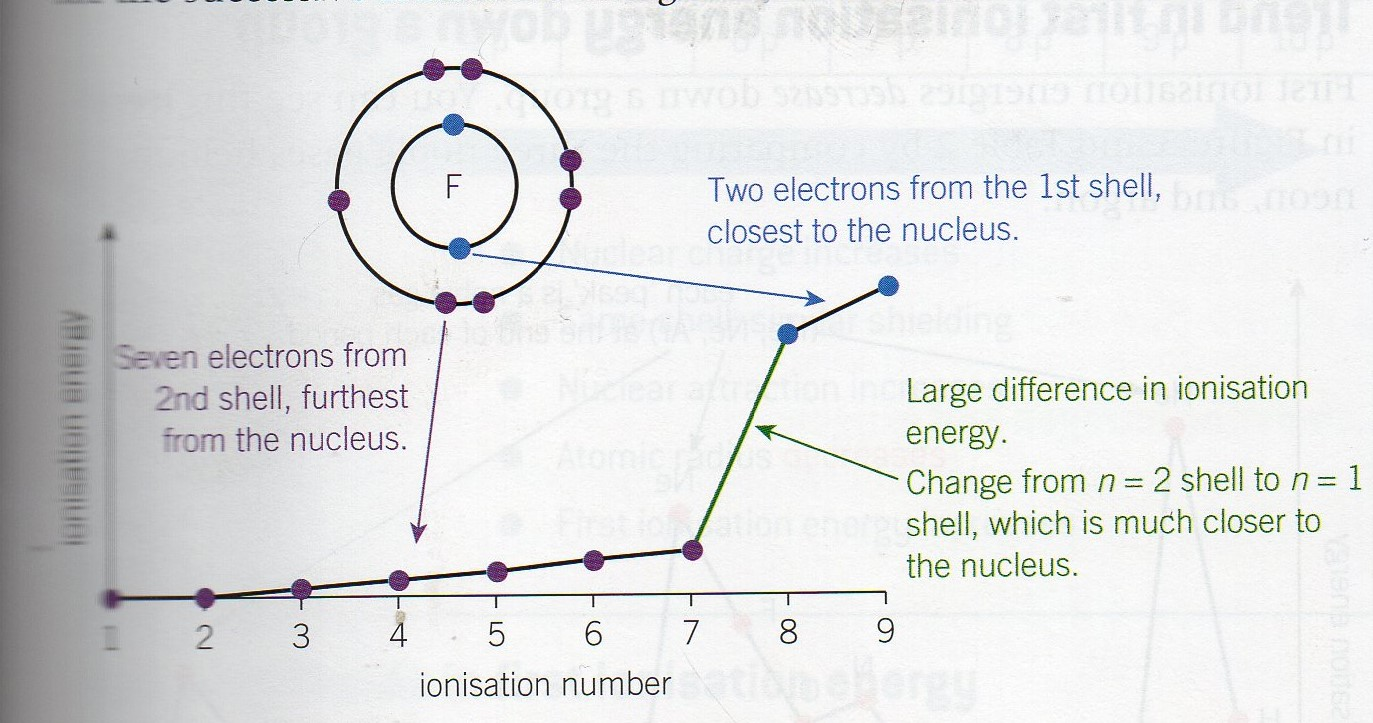
\includegraphics[scale=1]{ionisatione}
\end{center}
\paragraph{The large increase between the 7th and 8th}ionisation energies can be explained by the 1s shell being reached, which has the strongest attraction to the nucleus. This means that more energy is needed to remove electrons in this subshell.
\paragraph{You can make predictions from the successive ionisation energies.} These are the group of the element, the number of electrons in the outer shell and the identity of the element.
\subsection{Trends in ionisation energies}
\paragraph{There is a general increase in ionisation energies across a period.}However, there is a sharp decrease in first ionisation energy between the end of a period and the start of a new one(noble gases are peaks).
\begin{center}
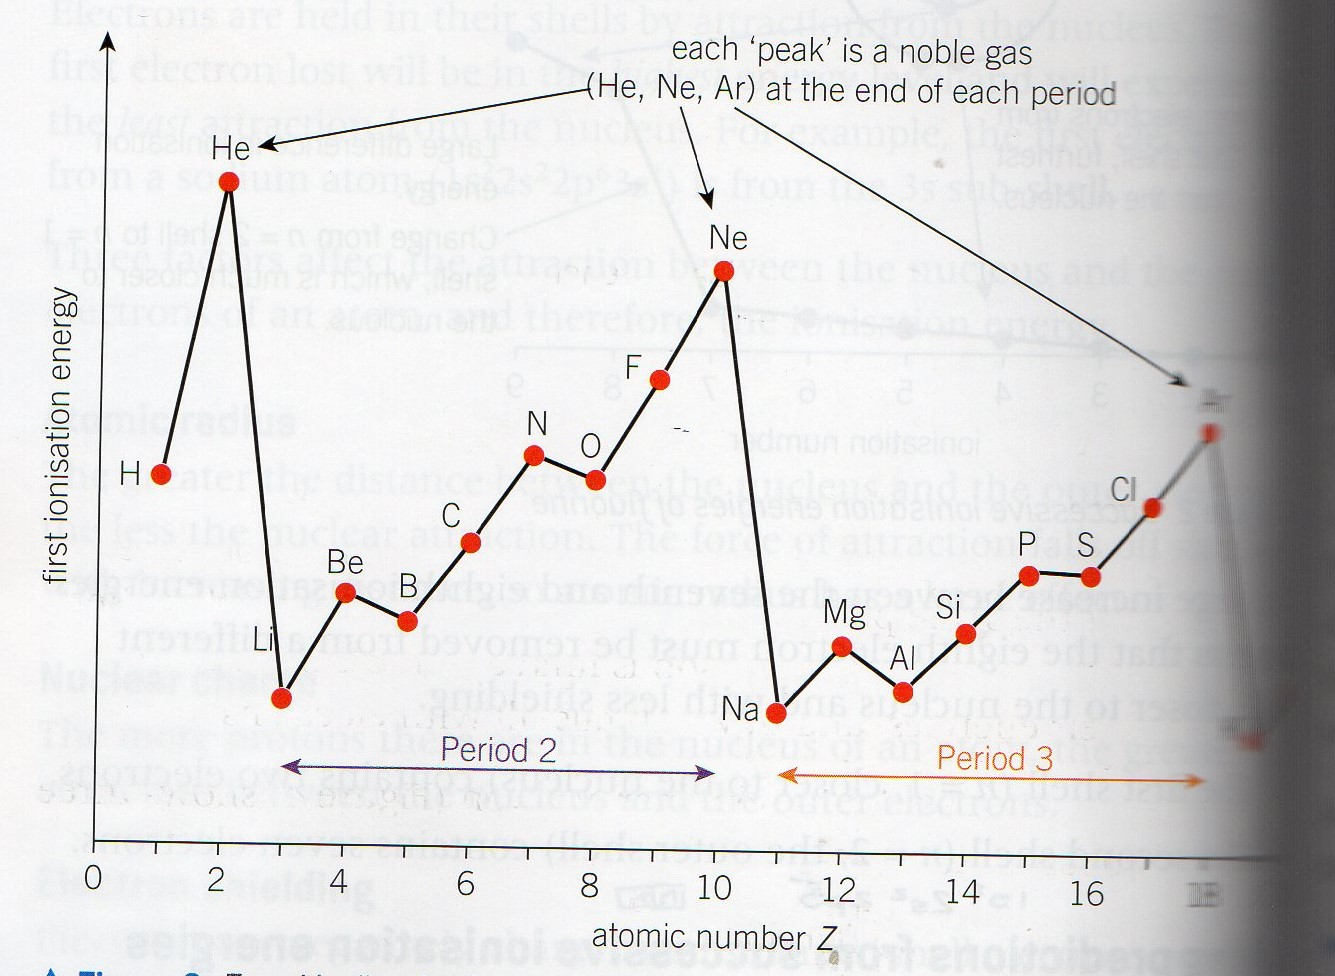
\includegraphics[scale=0.7]{periodio}
\end{center}
\paragraph{First ionisation energy decreases down all groups}because the atomic radius increases and electron shielding increases. Although nuclear charge increases, these effects outweigh it. 
\paragraph{First ionisation energy increases across periods.}This is due to similar levels of electron shielding as they are in the same shell.Next, there is a greater nuclear charge, increasing nuclear attraction as the atomic radius is smaller. This means that it is harder to remove electrons form elements.
\paragraph{Electrons in the same p sub-orbital repel each other. This makes it easier to remove an electron, decreasing first ionisation energy e.g. with N and O.}
\section{Periodic trend in structure 3.1.1}
	
	\paragraph{Metallic bonding} is the a ``strong electrostatic attraction between \textbf{fixed} cations (positive ions) and a sea of \textbf{delocalised} electrons".
	This bonding is between metal atoms and forms giant metallic lattices.
	\paragraph{Metals are able to conduct electricity} because of the sea of delocalised electrons created each metal donating its electrons to a shared pool of electrons.
	Metals are almost always \textbf{solid} at room temperature, except for mercury.
	This is because \textbf{metallic bonding is very strong}, but dependent on how many electrons the elements lose i.e. how positive cations are, as well as well as other factors.
    \paragraph{The melting point of metallic structures} is dependant upon the strength of the electrostatic attraction between cations and electrons. 
    Metals do not dissolve. This is even true with polar solvents as metals react rather than dissolving.
	
	\paragraph{Giant covalent lattices} are, unlike simple molecular lattices, atoms not molecules bonded by covalent bonds.
	This can make for some \textbf{incredibly strong compounds}.
	Carbon, boron and silicon are examples of atoms that can form giant covalent lattices.
	Carbon can form Diamond, graphite and graphene.
    \paragraph{Other than graphite and graphene, giant covalent lattices will not conduct electricity.}
	This is because the electrons are \textbf{immobile}. However graphite has a free electron per carbon atom. 
	These electrons join a sea of delocalised electrons and can move between the layers in the carbon.
	These mobile charge carriers are what allow graphite and graphene to be conductive.
	
	\paragraph{Solubility} Both metals and giant covalent lattices are, on the whole insoluble.
	In the case of metals, they may well react when in polar solvents not dissolve.
	In the case of giant covalent lattices, the bonding is far too strong to be broken by solvents.
	
	\paragraph{Graphene} is the latest wonder allotrope of carbon.
	It consists of a single layer of graphite, composed of hexagonally linked carbon atoms.
	It has the same electrical conductivity of copper and is the thinnest, strongest element ever made.
	The reason for its electrical conductivity is that it has, like graphite, delocalised electrons- as it doesn't use all electrons for bonding.
	These act as mobile charge carriers.
	
	There is potential for this to be used in micro-computing to replace silicone, this could serve to further decrease the size and cost of computer processors.
	
	\paragraph{Melting points} for giant metallic/covalent structures are very high.
	This means the following (for periods 2 and 3):
	\begin{itemize}
		\item As we move from groups 1 to 14 we see a rise in melting temperatures as these elements form \textit{giant structures}.
		\item A sharp drop is seen at group 14 to 15. This is because group 15-18 elements don't form giant structures.
		\item Group 15 to 18 are comparatively low. This is because are \textit{simple molecular structures}.
	\end{itemize}
\section{Group 2 -3.1.2}

	\paragraph{S sub-shell} Is filled in all the group two elements.
	This means that they contain two more electrons than the Nobel gas before it.Note that redox reaction are the most common ones involving Group 2 elements.In redox reactions these substances loose two electrons and from 2+ ions.The next part is just revisiting redox and so I will just summarise.You should know how group two elements from Mg$\rightarrow$Ba react with water, oxygen and weak acids.Just know that group 2 elements are oxidised by +2.
	
	\paragraph{Reactivity} increases as we go down the group because the group two elements in a reaction lose electrons.
	So as we learned before, as we move down the group the first (and in this case second) ionisation energies decrease due to greater shielding\footnote{Shielding is where electrons from other shells repel electrons in the outer shells.} and a greater atomic radius,reducing nuclear attraction.
e.g. \ch{CaO$_{(s)} + H2O$_{(l)}->Ca$^{2+}_{(aq)} + 2 OH$^-_{(aq)}}
\paragraph{Note that alkalinity increases if you shake Group 2 metals in water, going down the group.}This is because the solubility of OH$^-$ ions increases as you go down the group.Also,Ca(OH)2 is used in agriculture to neutralise acid soils and Mg(OH)2 and CaCO3 are used as ‘antacids’ in treating indigestion.
\section{The halogens 3.1.3}
	\paragraph{Boiling trends} in halogens are caused because of there existence as diatomic molecules.
	\textbf{The boiling point increases down the group} because of the \textbf{stronger London forces} (caused by more electrons to allow extra random motion causing induced dipoles).
\paragraph{Redox again} is found here. Much the same as all the others but this time they are oxidising agents.This is because they need only gain one electron to have the electron configuration of a noble gas.They form anions.
	
	\paragraph{Displacement reactions} occur when a significantly \textbf{more reactive chemical} is reacted with a compound containing a similar, but less reactive, compound.Using displacement reactions we can see that reactivity decreases down the group.
\paragraph{Halogen-halide displacement} The reactions are as follows,
	\begin{itemize}
		\item a chloride solution will not be displaced by bromine or iodine. This is because chlorine is the most reactive.
		\item a bromide solution will react when chlorine is added. It will turn orange as the Br$^-$ ions are displaced and so from Br$_2$,
		
			\ch{Cl2(aq) + 2 Br^-(aq) -> 2 Cl^-(aq) + Br2(aq)}
			However given that iodine is less reactive still there will be no reaction between \ch{I2} and bromide.
		\item As the least reactive iodide solution will be displaced by both chlorine and bromine to form a brown solution,
		
			\ch{Cl2(aq) + 2 I^-(aq) -> 2 Cl^-(aq) + I2(aq)}
			
			\ch{Br2(aq) + 2 I^-(aq) -> 2 Br^-(aq) + I2(aq)}
	\end{itemize}
	To tell apart the similar brown and orange we can add a non-polar solvent like cyclohexane to dissolve the halogen.
	When \ch{I2} is dissolved we can see the cyclohexane layer go a deep violet.
	
	\paragraph{The reason for decreasing reactivity} is that it is the opposite to group two.
	To gain an electron we need more attraction.
	As such more shielding and a grater atomic radius just cause less attraction to the electron and make it less reactive.
	
	\paragraph{Disproportionation} is what we call a reaction when the same element undergoes reduction and oxidation.
	This is illustrated by the following,
	\begin{itemize}
		\item The treatment of water with chlorine
		
		\ch{"\ox{0, Cl}" {}2(aq) + H2O(l) -> H "\ox{+1,Cl}" {}O(aq) + H "\ox{-1, Cl}" {}(aq)}
		
		As we can see, Chlorine has been both oxidised and reduced.
		
		\item The reaction of chlorine with cold, dilute aqueous sodium hydroxide,
		
		\ch{"\ox{0, Cl}" {}2(aq) + 2 NaOH(aq) -> Na "\ox{+1, Cl}" {}O(aq) + Na "\ox{-1, Cl}" {}(aq) + H2O(l)}
	\end{itemize}
	
	\paragraph{Water treatment} using chlorine is extremely useful.
	This is because chlorine kills bacteria.
	However, there are some hazards in using chlorine.
	Toxic chlorine gas and the risk of forming carcinogenic chlorinated hydrocarbons (when reacting with plant matter) and chloride ions can damage human tissue i.e. cancer.
	
	\paragraph{The Halide tests} are reactions used to test for halide ions in aqueous solution.
	This is done by adding aqueous silver ions (by using \ch{AgNO3}).
	The ionic equation is as follows (where X is any halide ion),
	
	\begin{center}
		\ch{Ag^+(aq) + X^-(aq) -> AgX(s)}
	\end{center}
	
	As we can see, this reaction creates a precipitate.
	Now we can derive the precise halide ion by looking at the colour of the precipitate.
	Chlorine will form a white precipitate, Bromine a cream and iodine yellow.
	
	Adding dilute aqueous ammonia will dissolve the precipitate AgCl, and by adding concentrated aqueous ammonia we dissolve both AgCl and AgBr.
	
\section{More tests 3.1.4}

	\paragraph{Three tests} you need to know for this section. They need to be done in the following order,
	\begin{enumerate}
		\item Carbonate (\ch{CO3^{2-}(aq)}) test
		\item Sulfate (\ch{SO4^{2-}(aq)}) test
		\item halide (\ch{Cl^-(aq)},\ch{Br^-(aq)} and \ch{I^-(aq)}) test
	\end{enumerate}
	
	\paragraph{Carbonate ions} are tested by adding a \textbf{dilute acid.} It is by the following ionic equations,
	\begin{center}
		\ch{CO3^{2-}(aq) + 2 H^+(aq) -> H2O(l) + CO2(g)}
	\end{center}
	As you can see \ch{CO2} is formed, which is gaseous. So if a \ch{CO3^-(aq)} ion is present we will see effervescence when we add it.
	We will see why we need to do this first.
	(remember to use an acid which will not interfere in the other two tests like \ch{NHO3}.
	
	\paragraph{Sulphate ions} are tested for by adding \textbf{\ch{Ba^{2+}(aq)}}. This is now by the following equations,
	\begin{center}
		\ch{Ba^{2+}(aq) + SO4^{2-} -> BaSO4(s)}
	\end{center}
	We see a white precipitate form (\ch{BaSO4(s)}).
	However this needs to be done after the carbonate test because \ch{Ba^{2+}} ions will form \ch{BaCO3(s)}, which is also a white precipitate.
	
	\paragraph{The halide tests} are mentioned above.
	
	\paragraph{Testing for ammonium ions} is simple. Just react with \textbf{warm aqueous NaOH},
	\begin{center}
		\ch{OH^-(aq) + NH4^+(aq) -> NH3(g) + H2O(l)}
	\end{center}
	So by adding NaOH we will see the solution effervesce if the NH$_4^+$ ions.
\subsubsection{Why is there a correct order?}
\paragraph{1. Carbonate test-}because when you add dilute acid, you are looking for effervescence. None of the other ions bubble when dilute acids are added to them, so it's OK to do it first.
\paragraph{2. Sulphate test-} when you add a solution containing Ba$^{2+}$, you are \textbf{hoping for a white precipitate} of BaSO$_4$.
\subparagraph*{BaCO$_3$ is white and insoluble in water,}therefore, if you perform a sulphate test on a carbonate, yyou will still get a white precipitate, giving false results.
\paragraph{3. Halide test-} when you add Ag$^+$ in AgNO$_3$, you are looking for a precipitate(yellow,cream or white).
\subparagraph*{Silver carbonate,Ag$_2$CO$_3$, and Silver sulphate, Ag$_2$SO$_4$ are both insoluble} in water,forming precipitates. This means you will get inaccurate results.
\subsubsection{What about a mixture of ions}
\begin{itemize}
\item\textbf{ Carbonate test}- add dilute HNO3 \textbf{until effervescence stops} if there is any, This makes sure there are no CO$_3^{2-}$ ions to react in the next test.(H2SO4 has sulphate ions and HCl has chloride ions)
\item \textbf{Sulphate test}- add \textbf{excess Ba(NO3)2} forming precipitate. \textbf{Filter} out the \textbf{precipitate}.Chloride ions would show up if BaX (halide) used.
\item Add AgNO3, therefore precipitate should form if previous steps done correctly.Add NH$_3$ to confirm what precipitate.
\end{itemize}
\subsubsection*{Test for cations}
\subsubsection{Test for ammonium \ch{NH4+}}
\paragraph{Aqueous ammonium ions and OH- ions(aq)}react to form \ch{NH3}gas when heated together.The equation is:
\begin{equation}
\ch{Nh4^+$_{(aq)} + OH^-$_{(aq)} -> NH3$_{(g)} + H2O$_{(l)}}
\end{equation}
\begin{enumerate}
\item NaOH$_{(aq)}$ added to solution containing ammonium ion
\item Ammonia gas produced- no bubbles as ammonia very soluble in water.
\item Mixture \textbf{warmed} and ammonia gas released.
\item You can smell the ammonia, but use moist \textbf{pH indicator paper}- turns blue.
\end{enumerate}
\section{Enthalpy 3.2.1}
\paragraph{Exothermic reactions are when}energy/heat is transferred to the surroundings from the system. Enthalpy change($\Delta$H) is negative because :
\newline $\Delta$H= H(\textbf{products})- H(\textbf{reactants}).
\paragraph{Endothermic reaction are when}energy is transferred from the surroundings into the system. The temperature of the surroundings decreases.
\begin{center}
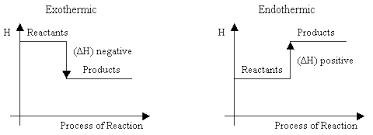
\includegraphics[scale=1]{energyprofile}
\end{center}
\paragraph{The minimum energy to break bonds in order to begin a reaction is the Activation Energy(E$_a$).}
\begin{center}
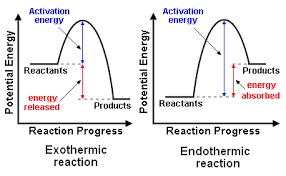
\includegraphics[scale=1]{activationenergy}
\end{center}
\paragraph{These are the standard conditions}needed for physical measurements such as enthalpy changes:
\begin{itemize}
\item Std. pressure: 100 kPa
\item Std. temp : 298K/25$\degree$C
\item Std. states: state that the chemical is in under these conditions.
\end{itemize}
formation,neutralisation,combustion
\paragraph{The enthalpy change of formation}is the enthalpy change that takes place when \textbf{1 mole} of a compound is \textbf{formed} \textbf{from} its \textbf{elements} in their \textbf{standard} states, under standard conditions.
\paragraph{The enthalpy change of combustion}is when \textbf{1 mole} of a \textbf{fuel} \textbf{fully reacts} with \textbf{oxygen} to form CO2 and H2O under \textbf{standard conditions} with all reactants and products in \textbf{std. states}.
\paragraph{The enthalpy change of neutralisation}is when \textbf{1 mole of water} is formed from the reaction of an \textbf{acid and an alkali} under standard conditions with all reactants and products in their \textbf{standard states}.
\begin{itemize}
\item  :\ch{Mg_{(s)} + 1/2 O2_{(g)}-> MgO_{(s)}} :formation
\item \ch{C4H10_{(g)} + 13/2 O2_{(g)} -> 4 CO2_{(g)} + 5H2O{(l)}}: combustion
\item \ch{H^+_{(aq)} + OH^-_{(aq)} -> H2O_{(l)}}: ionic for neut.
\item \ch{HCl_{(aq)} + NaOH_{(aq)} -> H2O_{(l)} + NaCl{(aq)} }
\end{itemize}
\subsection*{Bond enthalpies}
\subsubsection*{Average bond enthalpies}
\paragraph{Average bond enthalpy}is the amount of energy required to break \textbf{one mole} of a \textbf{specified} type of \textbf{bond} in a \textbf{gaseous} \textbf{molecule}. They are \textbf{always endothermic}- therefore values are +ve, but enthalpy of reaction can be -ve.
\paragraph{Bond breaking is endothermic, bond forming is exothermic.} The difference between the two determines if a reaction is exo/endothermic i.e. in an exothermic reaction, there would be more bond forming than bond breaking.
\begin{equation}
\Delta_rH= \Sigma(bond- enthalpies- reactants)-\Sigma(bond- enthalpies- products)
\end{equation}
\begin{center}
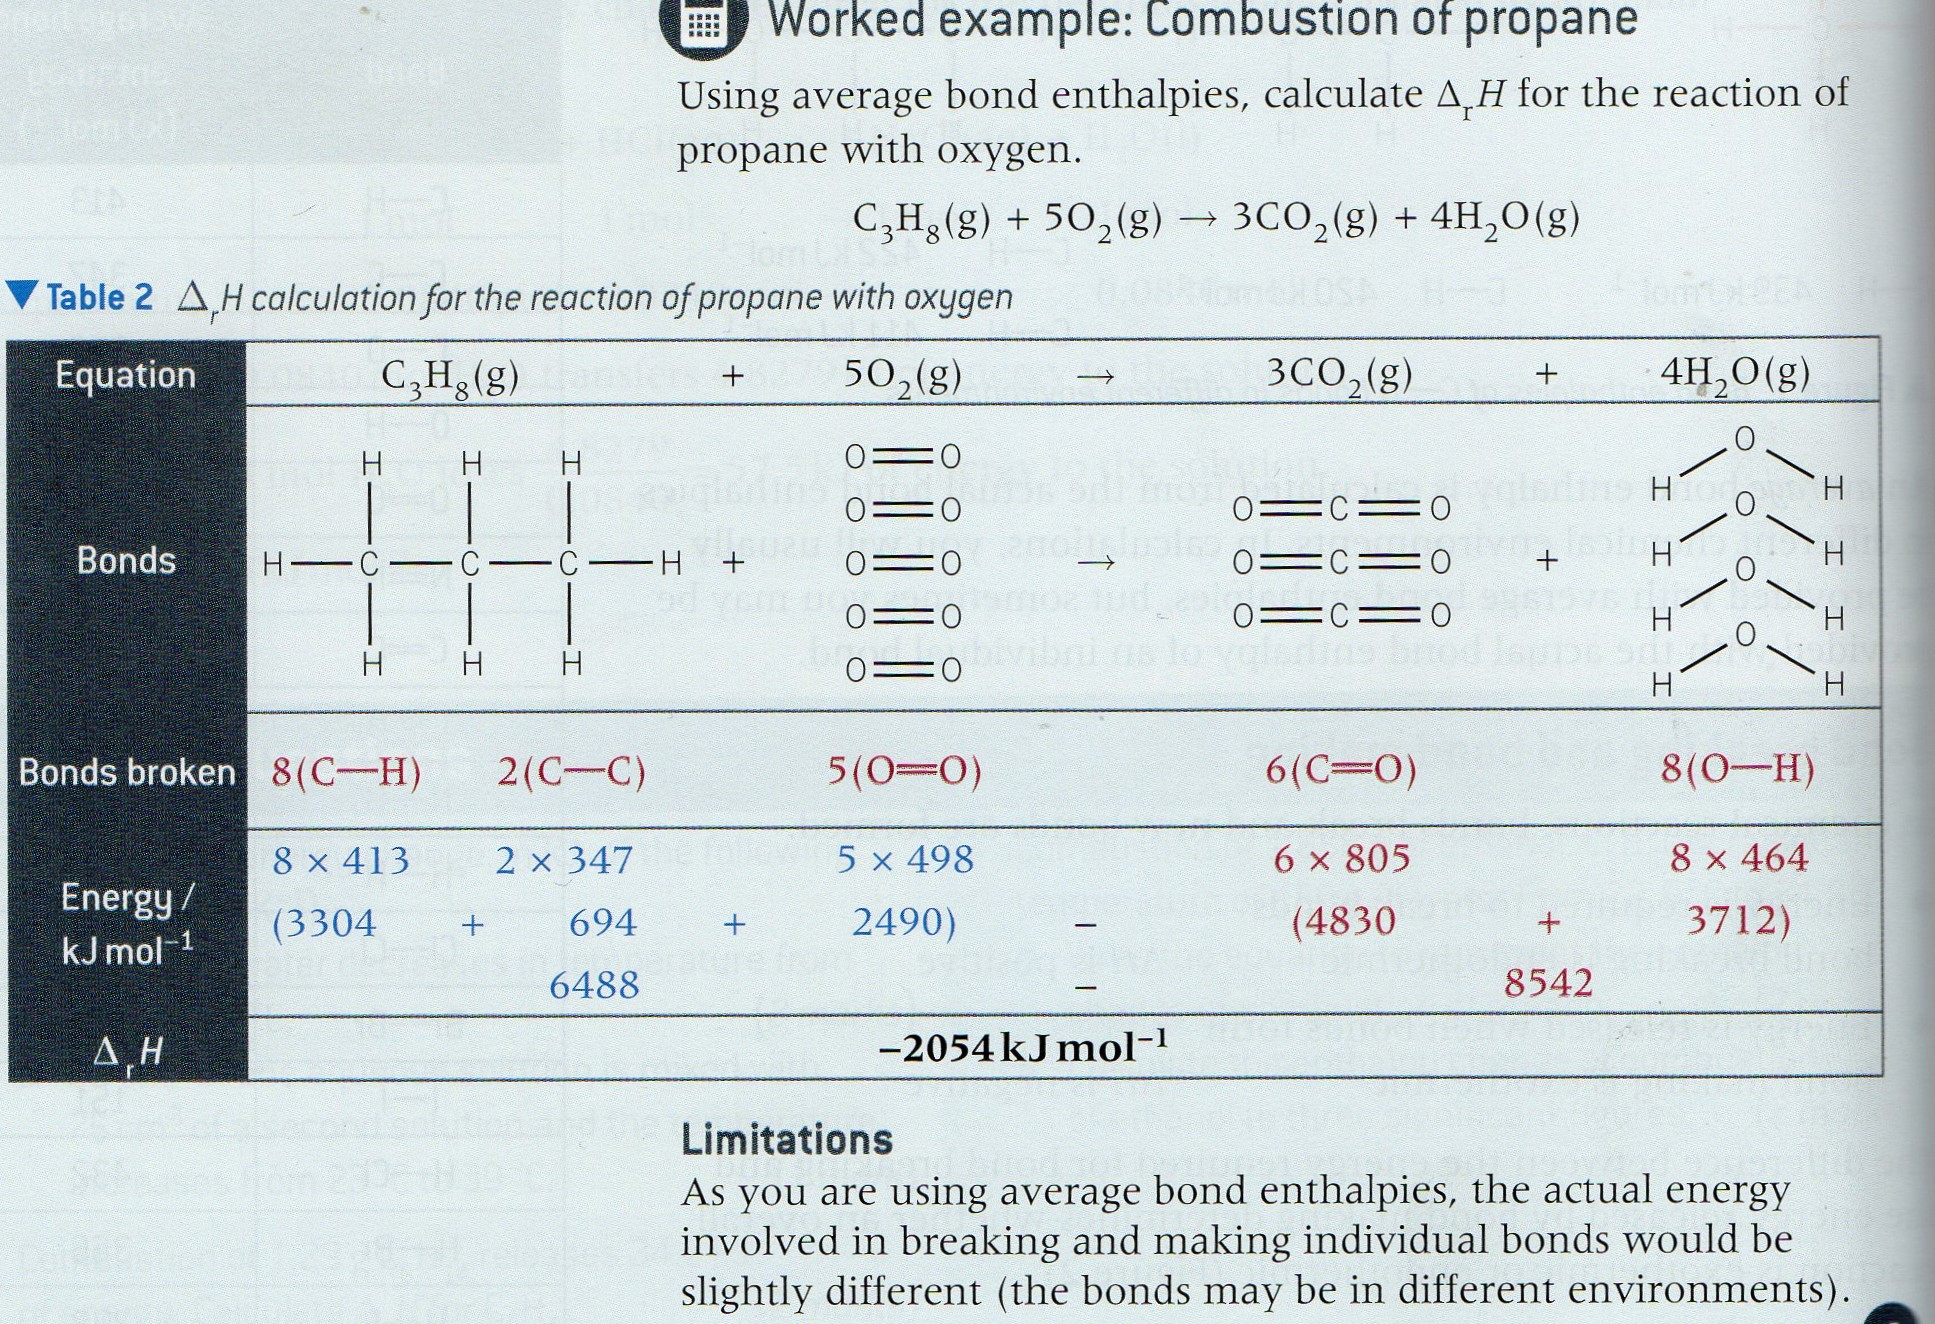
\includegraphics[scale=1]{avgbond}
\end{center}
\subsection{Hess' law and enthalpy cycles}
\paragraph{Hess' law allows enthalpy changes to be found indirectly.}It states that if a reaction can take place by 2 routes, and start and end conditions are the same, the enthalpy. It comes from the idea of conservation of energy.
\paragraph{You need to remember for}enthalpy change of \textbf{formation} \textbf{A+B=C} and for enthalpy change of \textbf{combustion}, \textbf{C+A=B}., where A is from reactant to product, B is elements to reactants and C is elements to product.
\newpage
\begin{center}
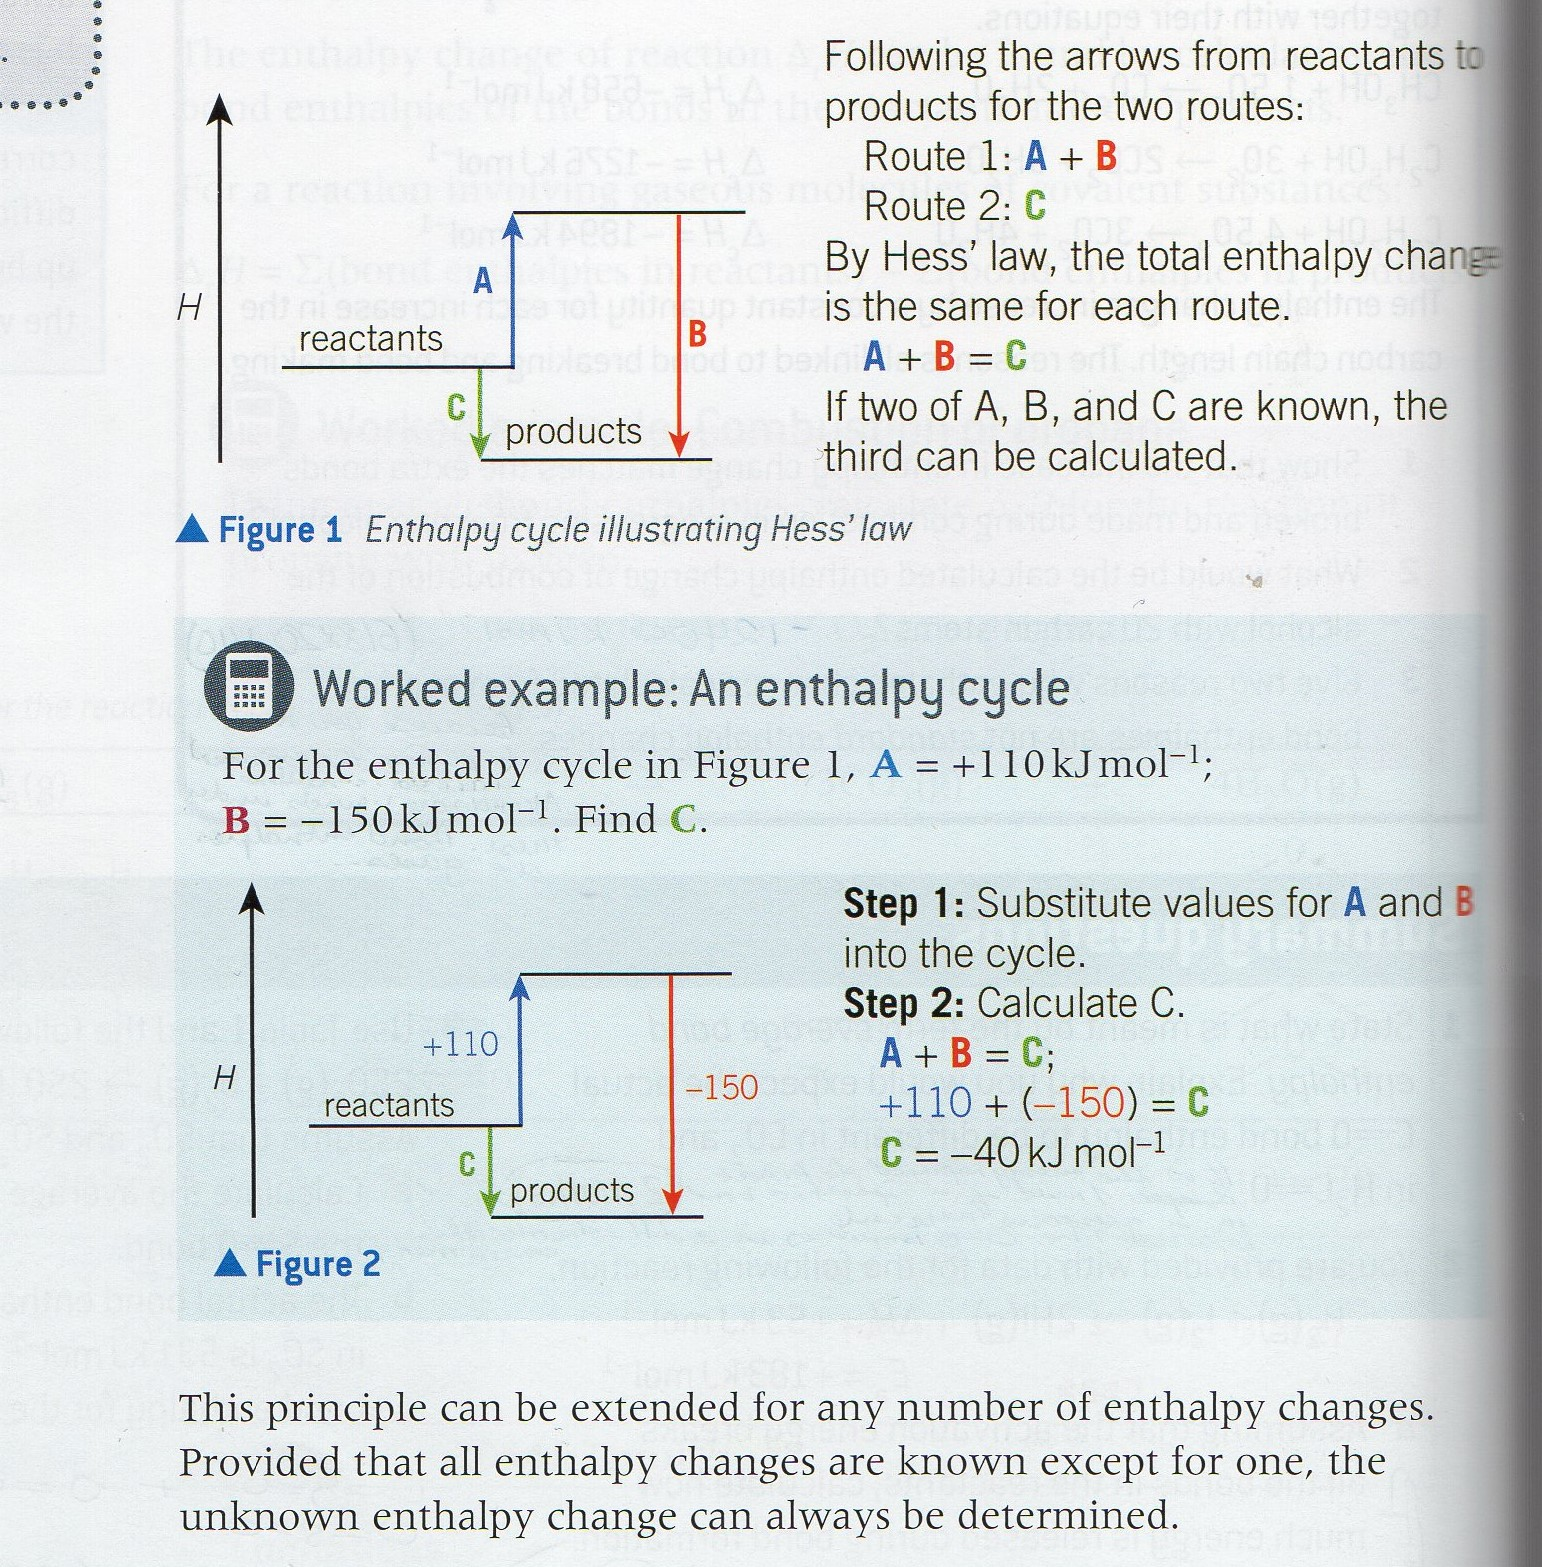
\includegraphics[scale=1]{cycles}
\end{center}


\section{Rates of Reaction 3.2.2}
	\paragraph{Collision} theory hasn't changed at all from GCSE.
	Sill we look at the microscopic consequences of pressure, concentration and temperature (kinetic energy) on individual molecules.
	Successful collisions are needed which is when the reactive atoms in a molecule collide.
	
	\paragraph{Catalysts} are substances that, when added to a chemical reaction, serve to increase the rate of reaction without reacting itself.
	
	This effect is achieved by the catalyst decreasing the required activation energy, thus providing a faster pathway for the reaction to take place.
	
	\paragraph{Homogeneous catalysts} refers to a catalyst that is in the same state as the reactants.
	This works by forming intermediate products.
	
	\paragraph{Heterogeneous catalysts} are catalysts which differ in state from the reactants.
	These act by a series of absorption and desorption.
	
	\paragraph{Catalysts} have massive importance in industry.
	They are used to reduce the amount of energy (in heat and pressure) in industrial reactions.
	This then reduces the amount of fossil fuels needing to be burnt, thus reducing \ch{CO2}.
	
	\paragraph{Measuring} rates of reaction can be done in many ways. This can involve measuring gas or mass over time.
	
	\paragraph{The Boltzmann distribution} is a frequency distribution used to predict the energy of molecules.
	The area under the curve represents the number of molecules with a given energy.
	The curve changes when the temperature rises (skews negativity). E$_a$ moves to the left when a catalyst is added.
	
\section{Chemical equilibrium 3.2.3}

	\paragraph{A dynamic equilibrium} exists in a closed system when the rate of the forward reaction is equal to the rate of the reverse reaction and the concentrations of reactants and products do not change.
	
	\paragraph{le Chatelier’s principle} states that ``When any system at equilibrium is subjected to change in concentration, temperature, volume, or pressure, then the system readjusts itself to (partially) counteract the effect of the applied change and a new equilibrium is established."
	
	Remember that catalysts do not affect the position of equilibrium as they only affect the activation energy, and the reaction goes both ways so this cancels out.
	
	\paragraph{Investigating equilibrium with concentration} is done by the following,
	
	\begin{center}
		\ch{2 CrO4^{2-}(aq) + 2 H^+(aq) <=> Cr2O7^{2-}(aq) + H2O(l)}
	\end{center}
	This reaction is sensitive to the acid concentration. Adding acid concentration will shift the point of equilibrium to the 'right'.
	We can see this because \ch{CrO4^{2-}(aq)} solution is yellow and \ch{Cr2O7^{2-}(aq)} solution is yellow.
	So by raising the concentration of the acid we see the solution got from yellow to orange.
	Procedure is as follows:
	\begin{enumerate}
		\item Add a solution of yellow potassium chromate to a beaker
		\item Add dilute sulfuric acid drop by drop until there is no further change in colour (orange).
		\item Add aqueous sodium hydroxide until there is no further change in colour (yellow).
	\end{enumerate}
	You have now witnessed equilibrium in action.
	\paragraph{Investigating equilibrium with temperature} is done by the following,
	
	\begin{center}
		\ch{[Co(H2O)6]^{2+}(aq) + 4 Cl^-(aq) <=> CoCl4^{2-}(aq) + 6 H2O(l)}
	\end{center}
	As temperature increases the reaction shifts right (in the endothermic direction) and vice-versa. This reaction can be done by the following steps,
	
	\begin{enumerate}
		\item Dissolve cobalt chloride in a boiling tube. Add a small quantity of hydrochloric acid. Then put the solution in ice to cool it until it turns pink (because \ch{[Co(H2O)6]^{2+}(aq)} solution is pink).
		\item Set up a boiling water bath and transfer the boiling tube. Wait until it turns blue (because \ch{CoCL4^{2-}} is blue).
		\item Transfer back to ice water and observe the change back to pink.
	\end{enumerate}
	And you have now witnessed a shift in equilibrium.
	
\section{The equilibrium constant, $K_c$ 3.2.3}

	\paragraph{Equilibrium constant} is calculated by,
	\begin{center}
		In the reaction $a$A + $b$B \ch{<=>} $c$C + $d$D
		\begin{equation}
			K_c = \frac{[\textnormal{C}]^c[\textnormal{D}]^d}{[\textnormal{A}]^a[\textnormal{B}]^b}
		\end{equation}
	\end{center}
	This requires a little explaining, The A, B, C and D values are the \textit{equilibrium} concentrations of the reactants (in mol dm$^{-3}$).
	
	Where $K_c = 1$ it indicates that the reaction is halfway between reactants and products.
	
	Where $K_c > 1$ it indicates that the position of equilibrium is shifted to the right (the products).
	
	Where $K_c < 1$ it indicates that the position of equilibrium is shifted to the left (the reactants).
	


\chapter{Core organic chemistry}
This module introduces organic chemistry and its important applications to everyday life, including current environmental concerns associated with sustainability.

\section{The basics 4.1.1}

	\paragraph{IUPAC rules} on the nomenclature of organic compounds is as follows,
		
	Firstly let me explain the parts of the name. Stem, prefix and suffix. The stem refers to the number of carbon atoms in the longest chain (just remember Monkeys Eat Peanut Butter + Greek); the prefix is in reference to a side chain (or a functional group); the suffix is added to indicate functional groups.
	
	We have three types of hydrocarbons, aliphatic, acyclic and aromatic. We will mostly focus on aliphatic hydrocarbons of which there are three homologous\footnote{A group of chemicals with the same functional group, differing by an addition of CH$_2$} series alkanes, alkenes and alkynes.
	
	\paragraph{Aliphatic} hydrocarbons are one which are joined in chains e.g,
	\begin{center}
		\chemfig{H-C(-[:90]H)(-[:270]H)-C(-[:90]CH_3)(-[:270]H)-C(-[:90]H)(-[:270]H)-H}
		
		\textit{2-methylethane}
	\end{center}
	
	\begin{samepage}
	\paragraph{Alicyclic} hydrocarbons join in cyclic shapes and look like this,
	\begin{center}
		\chemfig{*6(------)}
		
		\textit{Cyclohexane}
	\end{center}
	\end{samepage}
	
	\paragraph{Aromatic} hydrocarbons have benzene rings which contain all or some of the carbon atoms,
	\begin{center}
		\chemfig{\chemfig{**6(------)}}
		
		\textit{Benzene}
	\end{center}
	
	\paragraph{Functional groups (prefixes)} are as follows,

	\begin{center}		
	\begin{tabular}{c|c|c|c}
Functional group&Prefix&Suffix&Displayed \\ \hline \hline
carboxylic acids&none&-oic acid&\chemfig{-C(=[1]O)(-[7]OH)}\\ \hline
aldehydes&none&-al&\chemfig{-C(=[1]O)(-[7]H)}\\ \hline
ketones&none&-one&\chemfig{C-C(=[:90]O)-C}\\ \hline
alchols&hydroxy-&-ol&\chemfig{-OH}\\ \hline
amines&amino-&-amine&\\ \hline
ethers&alkoxy-&-ether&\\ \hline
fluorine&fluoro-&none&\\ \hline
chlorine&chloro-&none&\\ \hline
bromine&bromo-&none&\\ \hline
iodine&iodo-&none&\\ \hline
	\end{tabular}
	\end{center}
	
	I included a few more, I should imagine you only need the first 3 and the haloalkane ones (given that they are the ones in the textbook).
	
	\paragraph{Displaying formula} There are three ways to display chemical formula (for the exam). These being the following,
	
	\textit{General formula} is the simplest algebraic formula of a member of a homologous series. For example, for an alkane C$_n$H$_{2n+2}$.
	
	\textit{Structural formula} is the minimal detail that shows the arrangement of atoms in a molecule. We write out each alkile group\footnote{C atoms in the main chain} and there surrounding atoms. E.g. for 2,4-pentandione we have \ch{CH3COCH2COCH3}.
	
	\textit{Displayed formula} is where the full molecule is drawn so in the case of 2,4-pentandione,
	
	\begin{center}
		\chemfig{H-C(-[:90]H)(-[:270]H)-C(=[:90]O)-C(-[:90]H)(-[:270]H)-C(=[:90]O)-C(-[:90]H)(-[:270]H)-H}
	\end{center}
	
	\textit{Skeletal formula} is the simplified organic formula, shown by removing hydrogen atoms from alkyl chains, leaving just a carbon skeleton and associated functional groups. So in the case of 2,4-pentandione,
	
	\begin{center}
		\chemfig{[:-35.25]-[:35.25](=[:90]O)-[:-35.25]-[:35.25](=[:90]O)-}
	\end{center}
	
	\paragraph{Definition} time (and summary, straight from the horse's mouth),
	\begin{itemize}
		\item homologous series (a series of organic compounds having the same functional group but with each successive member differing by CH$_2$)
		\item functional group (a group of atoms responsible for the characteristic reactions of a compound)
		\item alkyl group (of formula C$_n$H$_{2n+1}$)
		\item aliphatic (a compound containing carbon and hydrogen joined together in straight chains, branched chains or non-aromatic rings)
		\item alicyclic (an aliphatic compound arranged in non-aromatic rings with or without side chains)
		\item aromatic (a compound containing a benzene ring)
		\item saturated (single carbon–carbon bonds only) and unsaturated (the presence of multiple carbon–carbon bonds, including C=C, C/C and  aromatic rings)
	\end{itemize}
	
	\paragraph{Structural isomers} are compounds with the same molecular formula but different structural formulae. Take, for \ch{C4H10}. Sound simple,
	\begin{center}
		\chemfig{-[:-35.25]-[:35.25]-[:-35.25]}
	\end{center}
	But now imagine a possible combination that could share the same molecular formula,
	\begin{center}
		\chemfig{-[:-30](-[:-90])-[:30]}
	\end{center}
	This is called a structural isomer. Both 2-methylpropane and butane are \ch{C4H10}. This is where structural formula and skeletal diagrams come in handy.
	
\section{Reaction Mechanisms 4.1.1}

	\paragraph{Homolytic fission} is where a covalent bond breaks and the electrons are shared evenly with each bonding 
atom receiving one electron from the bonded pair, forming two radicals.

	\paragraph{Heterolytic fission} is where a covalent bond breaks and the electrons are not shared evenly with one bonding atom receiving both electrons from the bonded pair.
	
	\paragraph{Radicals} are a species with an unpaired electron. We use a dot to show this, e.g. \ch{H3C-CH3 -> H3C "$\bullet$" {} + CH3 "$\bullet$" {}}. This being homolytic fission as each bonded atom receives one electron.
	
	\paragraph{Curly arrows} are used to describe the movement of an electron pair. They show either heterolytic fission or the formation of a covalent bond.
	
	\paragraph{Reaction mechanism diagrams} are used to show reaction mechanisms. They need to be sufficiently detailed, to show clearly the movements of an electron pair, with curly arrows and relevant dipoles.
	
\section{Alkanes 4.1.2}
	
	\paragraph{Alkanes} are saturated hydrocarbons containing single C–C and C–H bonds as $\sigma$-bonds (overlap of orbitals directly between the bonding atoms); free rotation of the $\sigma$-bond.
	
	\paragraph{A $\sigma$-bond} is the result of two overlapping orbital in. It is a single covalent bond.
	
	\paragraph{The bond angle} formed when a carbon atom has 4 $\sigma$-bonds is 109.5\degree .
	
	\paragraph{Trends in boiling points} are also obvious. The larger the molecule the more London forces there are at play. This means that the larger the molecule the more energy is needed to break the intermolecular forces and hence boiling the alkane. We also see the boiling point lower if the molecules branch. This is due to less surface area.
	
	\paragraph{Reactivity} of alkanes is low. This is because of the relative stability\footnote{High bond enthalpy} and very low polarity of the $\sigma$-bonds. 
	
	\paragraph{The combustion of alkanes} is seen everywhere. This is because fossil fuels like methane are alkanes. The longer the chain the more energy released per mole. The combustion reaction is as standard producing \ch{CO2} and \ch{H2O}.
	
	\paragraph{Alkanes and halogens} can react in the presence of UV radiation,
	\begin{center}
		\ch{CH4(g) + Br2(l) ->[UV] CH3Br(g) + HBr(g)}
	\end{center}
	However you need to know the mechanism of this reaction. It is as follows:
	\begin{enumerate}
		\item First the bond in the bromine molecule is broken up by homolytic fission \ch{Br-Br ->[UV] Br "$\bullet$" {} + "$\bullet$" {} Br}
		\item Next we have the propagation steps. This forms a chain reaction,
		\begin{enumerate}
			\item \ch{CH4 + Br "$\bullet$" {} -> "$\bullet$" {} + HBr}
			\item \ch{"$\bullet$" {} CH3 + Br2 -> CH3Br + Br "$\bullet$" {}}
		\end{enumerate}
		\item Finaly there is the termination, in which the two radicals collide forming a molicule with all the electron pairs. There are a number of ways this could happen.
		\begin{itemize}
			\item \ch{Br "$\bullet$" {} + "$\bullet$" {} Br -> Br2}
			\item \ch{"$\bullet$" {} CH3 + "$\bullet$" {} CH3 -> C2H6}
			\item \ch{"$\bullet$" {} CH3 + "$\bullet$" {} Br -> CH3Br}
		\end{itemize}
	\end{enumerate}
	
\section{Basics in Alkenes 4.1.3}

	\paragraph{Alkenes} are unsaturated hydrocarbons containing a C=C bond comprising a $\pi$-bond (sideways overlap of adjacent p-orbitals above and below the bonding C atoms) and a $\sigma$-bond (overlap of orbitals directly between the bonding atoms). The $\pi$ bonds prevent the C=C bond from rotating freely. I will explain later.
	
	\paragraph{The structure} is trigonal planar with the bonding angle around each C=C alkenes is 120\degree .
	
	\paragraph{Stereoisomers} are compounds with the same structural formula but with a different arrangement in space. We look at E/Z isomerism. This is when we see stereoisomers are formed due to a restriction of rotation around the C=C group.
	
	\paragraph{cis–trans isomerism} special case of E/Z isomerism in which two of the substituent groups attached to each carbon atom of the C=C group are the same.
	
	\paragraph{Cahn–Ingold–Prelog (CIP) priority rules} are used to strictly define EZ isomers. It is based on 'priority' of the atoms bonded to the C=Cs. The 'priority' is down to the relative height of atomic number.
	\begin{center}
		\chemfig{C(-[:120]CH_3)(-[:-120]H)=C(-[:60]H)(-[:-60]CH_3)}
	\end{center}
	Will be an E isomer because C has a higher atomic number than H.
	\begin{center}
		\chemfig{C(-[:120]H)(-[:-120]CH_3)=C(-[:60]H)(-[:-60]CH_3)}
	\end{center}
	And be a Z isomer.

\chapter{Rates of reactions}
\section{Order, rate equation and rate reactions}
\subsection{Rate of reaction}
\paragraph{Rate of reaction is measured} by observing \textbf{changes over time}. It is basically measuring quantity produced/time e.g. cm$^3 s^{-1} $. In this chapter, you will mainly be dealing with concentration, so knowing the standard unit for it is important(mol $ dm^{-3}$).
\paragraph{Chemists use shorthand} to describe the concentration of compounds. This notation is [A], where A is the compound, and the square brackets mean 'concentration of'.
\begin{equation}
Rate \propto [A]^n - \textnormal{rate is directly proportional to the concentration of A}
\end{equation}
\subsection{Orders of reaction}
\paragraph{The rate of reaction}will often increase as the concentration is increased. It is directly proportional to the concentration raised to a power i.e.
\begin{equation}
rate\propto [A]^n
\end{equation}
The power is the order of reaction with respect to the concentration of the compound in the square brackets.
\subsubsection{Zero order}
\paragraph{This is when}\ch{rate=[A]^0}, meaning that a change in concentration has no effect on the rate of reaction. This is due to anything to the power of 0=1. 
\subsubsection{First order}
\paragraph{This is when}\ch{rate=[A]^1}. Essentially, what happens to the concentration happens to the rate i.e. concentration x2 means rate x2.
\subsubsection{Second order}
\paragraph{This is when}\ch{rate=[A]^2}.So when concentration doubles, rate x$2^2=4$. Basically the rate is the square of the change in concentration.
\subsection{Rate equation and rate constant}
\paragraph{The rate equation is}$rate=k[A]^n[B]^m$. The overall order can be found by adding the powers together. When a question says both concentrations are changed, you use the overall order to find the rate.
\paragraph{The units of the rate constant}are usually \ch{moldm^{-3}s^{-1}}. However,this can be derived by rearranging the rate equation to make k the subject as this is the rate constant. It is useful to remember that the concentrations are measured in \ch{moldm^{-3}}.
\subsection{Determining orders from experimental results}
\paragraph{The best way}to learn this is by doing past paper question. Some great resources can be found on: pastpapers.com; physicsandmathstutor.co.uk or http://www.a-levelchemistry.co.uk/.
\paragraph{The questions}will usually contain a table with the headings: Experiment, Concentration of respective elements and the initial rate. The way to go about these questions is by first seeing how the concentration change between experiments e.g. x2. Then look at initial rate. See how this changes to determine the rate e.g. if it's x4, this would be second order.
\begin{center}
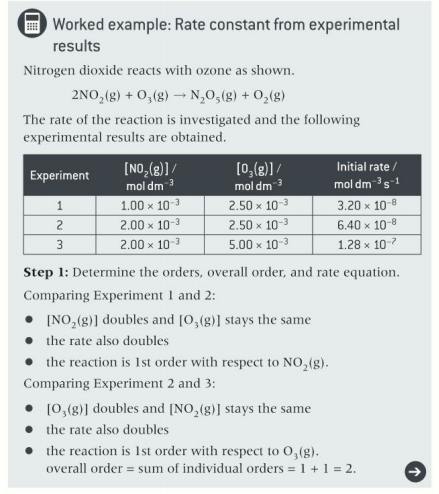
\includegraphics[scale=0.5]{workedorder.png}
\end{center}
\newpage
\section{Concentration-time graph}
\paragraph{You can measure rates}by looking for a \textbf{change} in mass or by gas collection in a certain \textbf{time}. You can also use a colorimeter if some of the compounds are coloured.
\subsection{Concentration-time graph}
\paragraph{The gradient of the concentration-time graph} is the rate of reaction.The order of reaction can be deduced from the shape of the graph.
\subsubsection{Zero order}
\paragraph{This graph slopes down}i.e. it has a negative gradient. The line is straight meaning that the rate is constant as concentration falls over time(as reactants used up). The gradient of the line is the rate constant-k.
\subsubsection{First order}
\paragraph{This graph is a downward-sloping curve}.The gradient decreases over time,slowing the reaction down. The \textbf{half-life}( \textit{time taken for concentration to halve}) is constant.
(INSERT GRAPHS WHEN BOTHERED)
\subsubsection{Second order}
\paragraph{This graph is steeper at the beginning than the first order.}However, it tails off more slowly
\subsection{Half-life}
\paragraph{Half-life,}which can be represented by $t_{1/2}$ is the time taken for half of the reactant to be used up. First order reactions halve the concentration every half life. The curve is exponential, showing \textbf{exponential decay}
\subsubsection{Determination of rate constant from rate}
\paragraph{You can draw a tangent to the curve}on a concentration-time graph.This will give you the rate of reaction. Then, you insert this into your re-arranged rate equation,where k is the subject.This should give you the rate constant, all you need to do is figure out the units.
\paragraph{You can also use an awesome formula:}\begin{equation}
k=\frac{\textnormal{ln}2}{t_{1/2}}
\end{equation}
This method is more accurate than drawing a tangent.
\section{Rate-concentration graphs and initial rates}
\paragraph{Always be careful to check the axes of your graph.}Here, the rate is on the left and concentration along the bottom. Normally, as concentration increases, so does rate due to kinetics i.e. more particles etc. Therefore the curves usually\textbf{slope up} rather than down.
\subsection{Orders from shapes}
\subsubsection{Zero order}
\paragraph{The gradient is 0,}meaning there is no slope. Rate is not affected by a change in concentration( a visual representation of its definition).The y-intercept gives you the rate constant-k.
\subsubsection{First order}
\paragraph{This is a upward-sloping straight-line graph}beginning at the origin. This is because when concentration is 0, rate is zero. The rate constant her is the gradient of the line.
\subsubsection{Second order}
\paragraph{This is an upward sloping curve.}Therefore the gradient constantly increases. It also means that the rate constant cannot be worked out directly by the curve. Instead, you need to \textbf{plot a second graph} of the rate against $[A]^2$ (concentration squared). This will give you a straight line graph through the origin, where the gradient is k.
\subsection{Initial rates method}
\paragraph{The initial rate}is the instantaneous rate when t=0.It can be measured by drawing a tangent where t=0 on a concentration-time graph.
\paragraph{A clock reaction}is a more convenient method of obtaining the initial rate. It is done by measuring time from the beginning of an experiment to a visual change. this will often be a precipitate or colour.
=======
\chapter{Physical chemistry and transition elements}



\end{document}